%************************************************
\chapter{Evaluation}\label{ch:evaluation}
%************************************************
This chapter evaluates the system proposed in \autoref{ch:design}. An implementation of this system can be found in \autoref{sec:demo_app}.  This chapter starts by evaluating this implemented system. Furthermore, \autoref{sec:eval_k} analyses the consequences of the sub sampling by showing the accuracy and CPU usage of the system.

\section{Demo app evaluation} \label{sec:demo_eval}
The demo application proposed in \autoref{sec:demo_app} consists of 9 containers, which are divided into three groups:
\begin{itemize}
    \item \textbf{Web-service} (3 containers): For receiving internal requests and generating CPU load.
    \item \textbf{Request-service} (3 containers): For generating the requests for the web-services.
    \item \textbf{Cassandra} (3 containers): For showing communication on a single node and generating a high memory consumption.
\end{itemize}

\noindent
The demo application is distributed over three nodes. An overview of these three nodes can be found in \autoref{tab:node_stats}. The containers per node can be found \autoref{fig:demo_app}.

\begin{table}
    \centering
    \begin{tabular}{l|lrr}
        Virtual Machine &IP & Cores & RAM \\ \hline
        Supernode & 10.164.0.2 & 1 & 3.9 GB \\
        Node 1 & 10.164.0.3 & 1 & 3.6 GB \\
        Node 2 & 10.164.0.7 & 2 & 7.3 GB \\
    \end{tabular}
    \caption{Overview of the nodes in the demo application}
    \label{tab:node_stats}
\end{table}

\begin{figure}
    \centering
    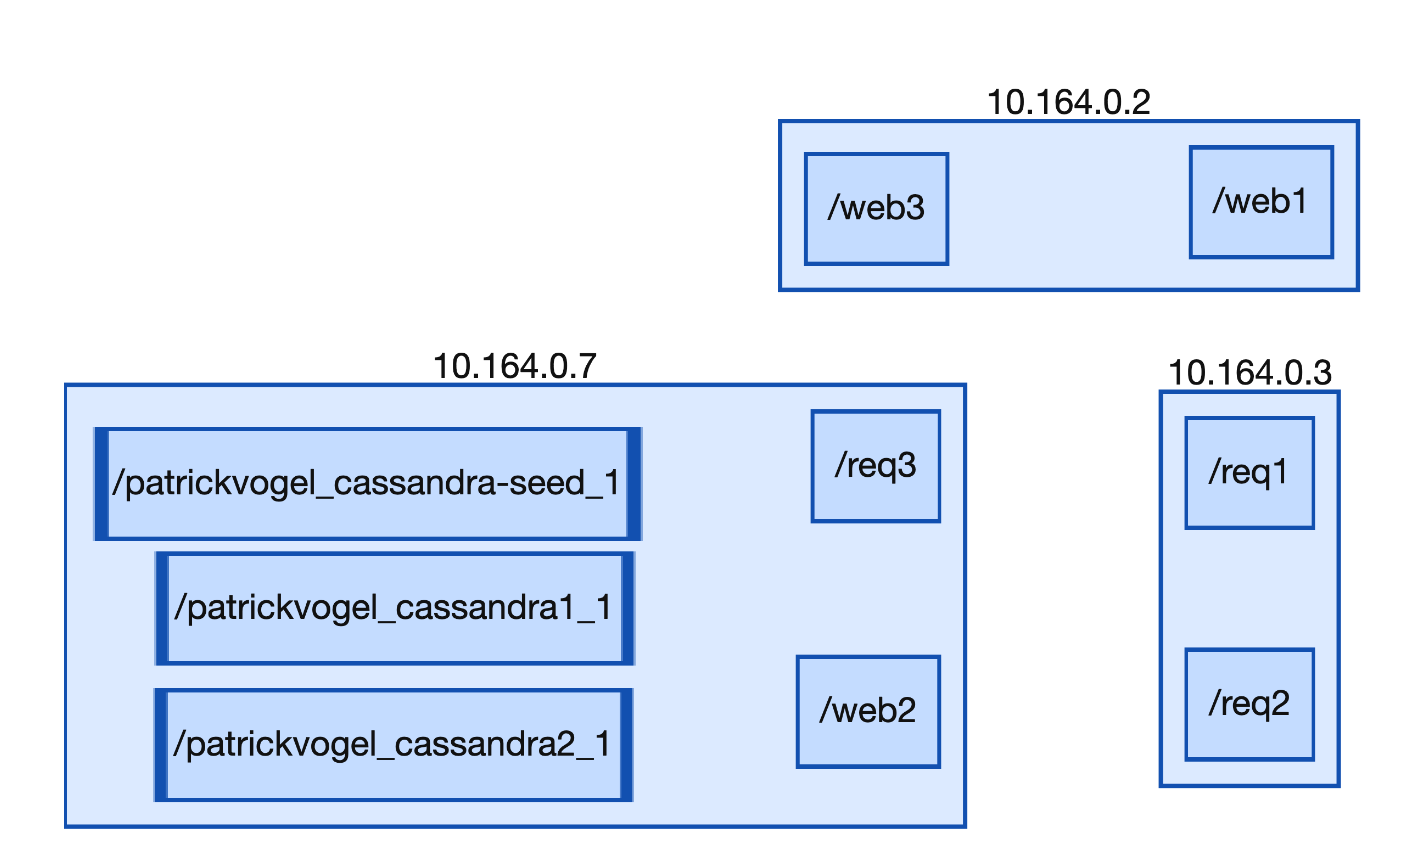
\includegraphics[width=\textwidth]{gfx/demo_app}
    \caption{All containers in the demo application}
    \label{fig:demo_app}
\end{figure}

\noindent
Interesting about this demo application is that it is easy to evaluate the cost model of the system. The supernode consumes almost all its CPU resources, but barely uses memory. Node 1 is low on memory and CPU, and can therefore be used to see how the waste is distributed. Node 2 consumes a lot of memory, but barely uses CPU. For a time period of one hour, the CPU usage is presented in \autoref{fig:demo_cpu}. From this figure, we conclude that the assumptions made above are correct. Note that the unit of the CPU usage is `CH', which means `core hour'. This represents $n_\text{CPU}$ from \autoref{eq:p}.


\section{Internet traffic accuracy evaluation} \label{sec:eval_k}
This section provides a small research about the accuracy of the internet traffic monitoring. In order to do so, a supernode was deployed to monitor two local containers. One container acting as a web-service, and one container continuously sending requests. The command for collecting all values can be found below:

\begin{lstlisting}[language=bash, caption=Docker-compose]
git clone htts://github.com/dadvisor/util
./util/accuracy.sh
\end{lstlisting}

\noindent
The idea behind this evaluation is to allow only one container to communicate with the web-service. By doing so, the total amount of data that a container sends is equivalent to its internal amount of data. Thus, the following variables should hold the same value:
\begin{itemize}
    \item \textbf{network\_container\_total}: This metric receives a value by scraping data from cAdvisor.
    \item \textbf{bytes\_send\_total}: This metrics has a key-value pair with both `src' and `dst'. This is the amount of data sent between the source container and the destination container by reading the Tcpdump data.
\end{itemize}

\noindent
By analysing the rate (per-second average rate of increase) over a time period of one hour, the accuracy can be determined. This can be expressed as the ratio between the two variables above. A perfect estimation would therefore result in a value of 1. The Prometheus query for analysing the accuracy is presented below.

\begin{verbatim}
rate(network_container_total[5m]) / on (src) 
rate(bytes_send_total[5m])
\end{verbatim}

\noindent
The evaluation has been made for different K values, as proposed in \autoref{sec:decisions}. The data obtained for $K = 3$ can be found in \autoref{fig:network_traffic_accuracy}. This figure shows the accuracy of the network traffic monitoring evaluation. Note that this figure shows several spikes, which is due to the difference update frequency of 
both variables. Therefore, the minimum and maximum value represent the boundaries of the accuracy. Furthermore, the accuracy is summarized by computing the average. The results for different K values can be found in \autoref{tab:accuracy_results}.

\begin{figure}
    \centering
    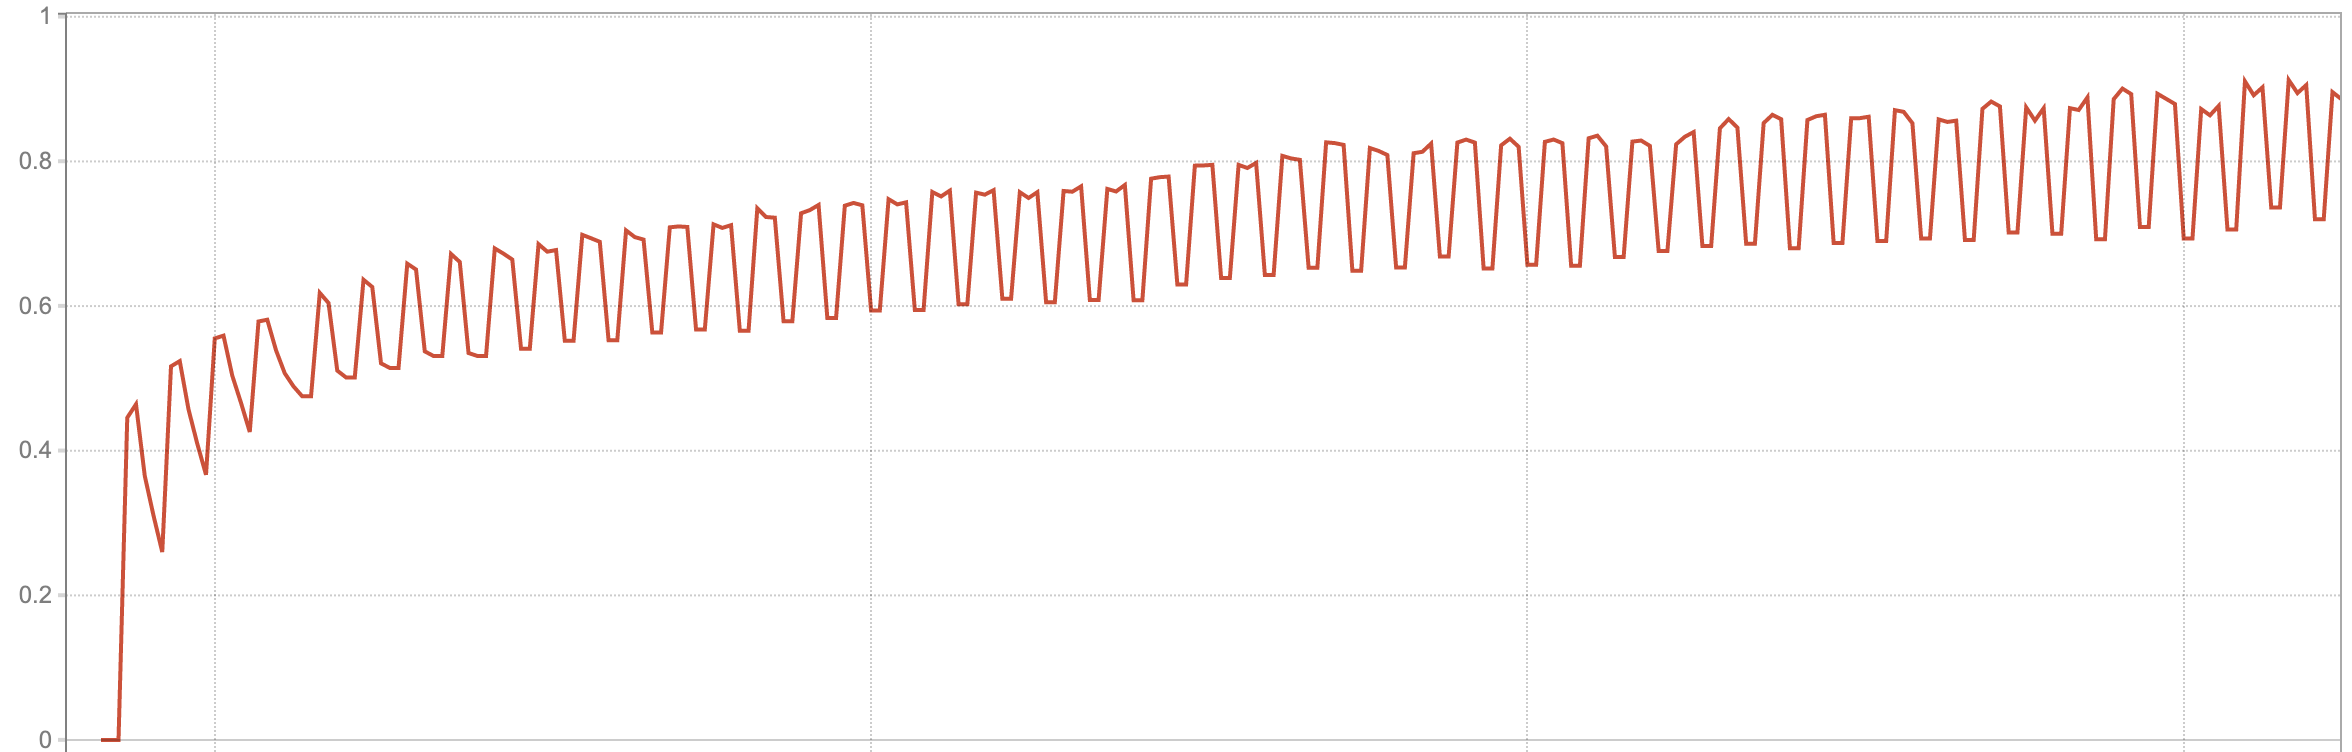
\includegraphics[width=\textwidth]{gfx/traffic_network_accuracy}
    \caption{Network traffic accuracy}
    \label{fig:network_traffic_accuracy}
\end{figure}

\begin{table}[ht]
    \centering
    \begin{tabular}{r|rrr|r}
        \multirow{2}{*}{K-value} & \multicolumn{3}{|c|}{Accuracy} & \multirow{2}{*}{CPU Usage} \\
        & Min & Max & average & \\ \hline        
        0 & 0.53& 1.22& 1.10& 9\% \\
        3 & 0.52& 1.04& 1.00& 4\% \\
        6 & 0.95& 1.74& 1.66& 3\% \\
        9 & 0.53& 1.29& 1.05& 3\% \\
        12& 0.93& 1.33& 1.10& 2\% \\
        15& 0.51& 1.11& 1.01& 2\% \\        
    \end{tabular}
    \caption{Network traffic accuracy results for different K-values}
    \label{tab:accuracy_results}
\end{table}

\subsection{Conclusion}
From \autoref{tab:accuracy_results} it can be concluded that there is not much variation in the accuracy across different K-values. A reason for this, is the fact that the network communication is not enough randomized. Thus, with a constant flow of traffic, the prediction of amount of network communication is too trivial.\\

\noindent
What can be concluded from this table, is the fact that the CPU usage drops if the K-value increases. This is due to a longer sleeping period. However, this number is not very accurate, as the analyses is performed on a single node. Therefore, the overhead of communicating with other nodes is not evaluated.